\chapter*{Distribuições de variáveis aleatórias e Movimento Browniano}
Serão descritos os algoritmos implementados, seus resultados em forma gráfica e algumas observações que conseguimos obter baseados na análise dos gráficos. Entre essas observações podemos citar: relação entre aumento do número de barras e pontos nos intervalos das variáveis aleatórias, mudanças na semente aleatória e na quantidade de pontos do movimento Browniano. Implementamos em C um algoritmo que gera números pseudo-aleatórios %(\ref{GeradorPseudoAleatoriosFONTE}), este algoritmo é um gerador multiplicativo pois o termo de soma na fórmula é zero. 

Implementamos em C um algoritmo %(\ref{d_Uniforme}) que satisfaz a distribuição uniforme, cuja Função densidade probabilidade (FDP) é dada por:
\begin{equation}
Fdp(X) = \frac{1}{|b-a|}
\end{equation}
\begin{figure}[!htb]
\centering
\begin{minipage}[b]{0.9\linewidth}
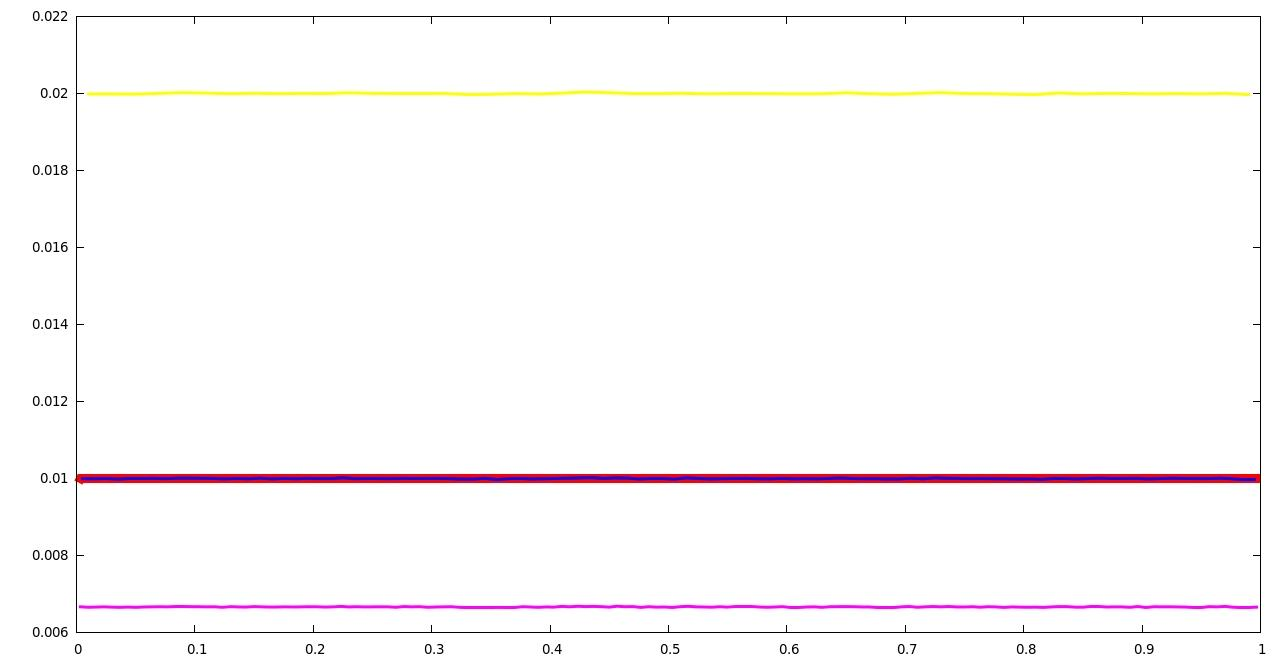
\includegraphics[width=\linewidth]{./img/Distribuicoes/uniVarNumBar.jpg}
\caption{Variação no número de barras da distribuição uniforme.}
\label{figUniformeBar}
\end{minipage} \hfill
\end{figure}
\begin{figure}[!htb]
\centering
\begin{minipage}[b]{0.9\linewidth}
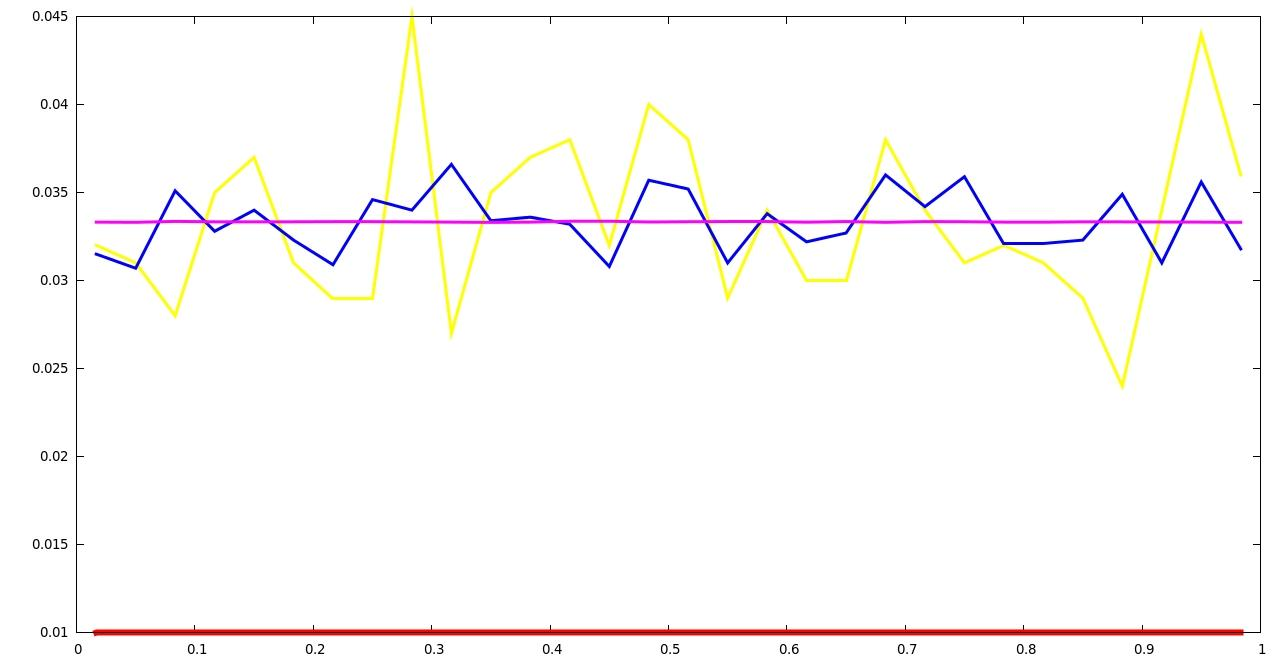
\includegraphics[width=\linewidth]{./img/Distribuicoes/uniVarNumPts.jpg}
\caption{Variação no número de pontos da distribuição uniforme.}
\label{figUniformePt}
\end{minipage} \hfill
\end{figure}


As curvas: vermelha e preta nas figuras (\ref{figUniformeBar}) e (\ref{figUniformePt}) representam variáveis aleatórias satisfazendo uma distribuição uniforme exata. Para plotar essas curvas foi utilizada a probabilidade da variável aleatória assumir um valor qualquer em um intervalo, tal probabilidade é dada pela frequência relativa:
\begin{equation}
f(x) = 0.01.
\end{equation}
Após analisar a figura (\ref{figUniformeBar}), constatamos que a diminuição do número de barras faz a distribuição uniforme se deslocar em direção oposta ao eixo X, já o aumento do número de barras  faz a curva se deslocar em direção ao eixo X. Pode-se verificar essa asserção comparando as curvas: vermelha (ideal), amarelo (50 barras) e rosa (150 barras).

Após análisar a figura (\ref{figUniformePt}) observamos que a acurácia das curvas aumenta ou diminuí (em relação a curva vermelha) de acordo com o aumento ou redução do número de pontos utilizados para plotar as curvas. Para verificar esta asserção pode-se comparar as curvas: amarela (1000pts), azul escuro (10000pts) e rosa ($10^{8} pts$), observa-se que a curva rosa (que possuí maior acurácia e número de pontos que a outras) possuí um comportamento mais próximo da curva vermelha (ideal).

Implementamos em C um algoritmo %(\ref{d_Exponencial}) que satisfaz a distribuição exponencial, ondeé a média , cuja FDP  é:
\begin{equation}
Fdp(X) = \lambda e^{-\lambda x}.
\end{equation}

\begin{figure}[!htb]
\centering
\begin{minipage}[b]{0.9\linewidth}
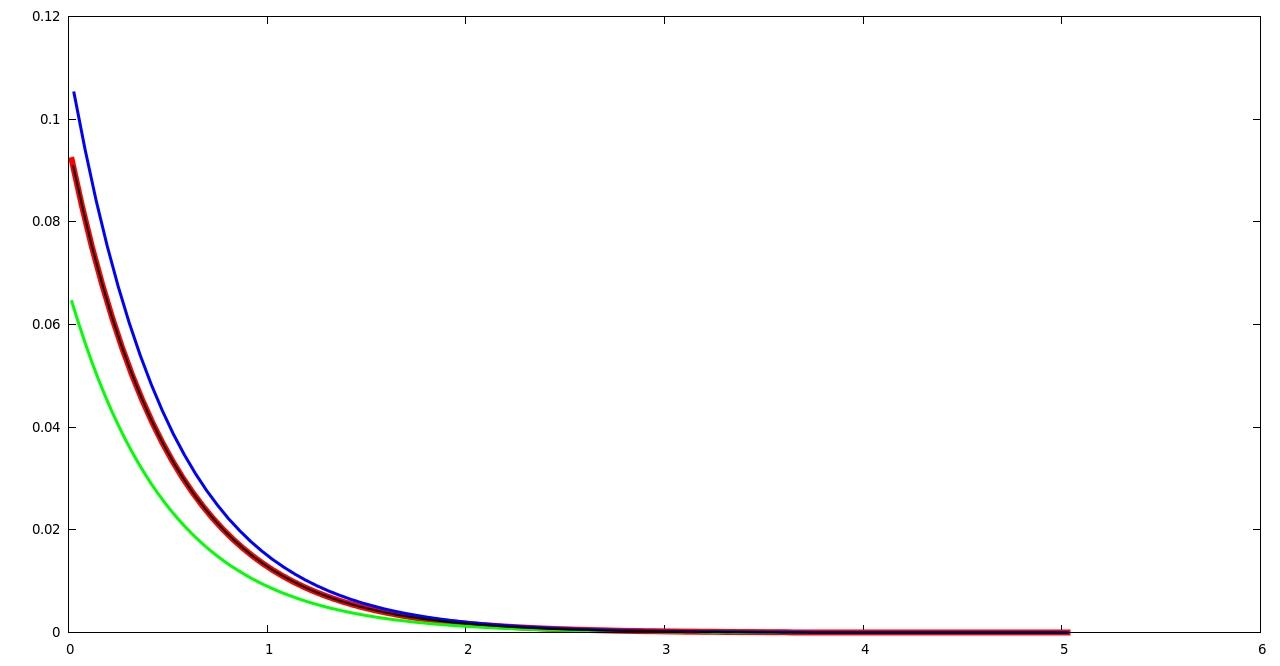
\includegraphics[width=\linewidth]{./img/Distribuicoes/expVarBarr.jpg}
\caption{Variação no número de barras da distribuição exponencial.}
\label{figExpBar}
\end{minipage} \hfill
\end{figure}

\begin{figure}[!htb]
\centering
\begin{minipage}[b]{0.9\linewidth}
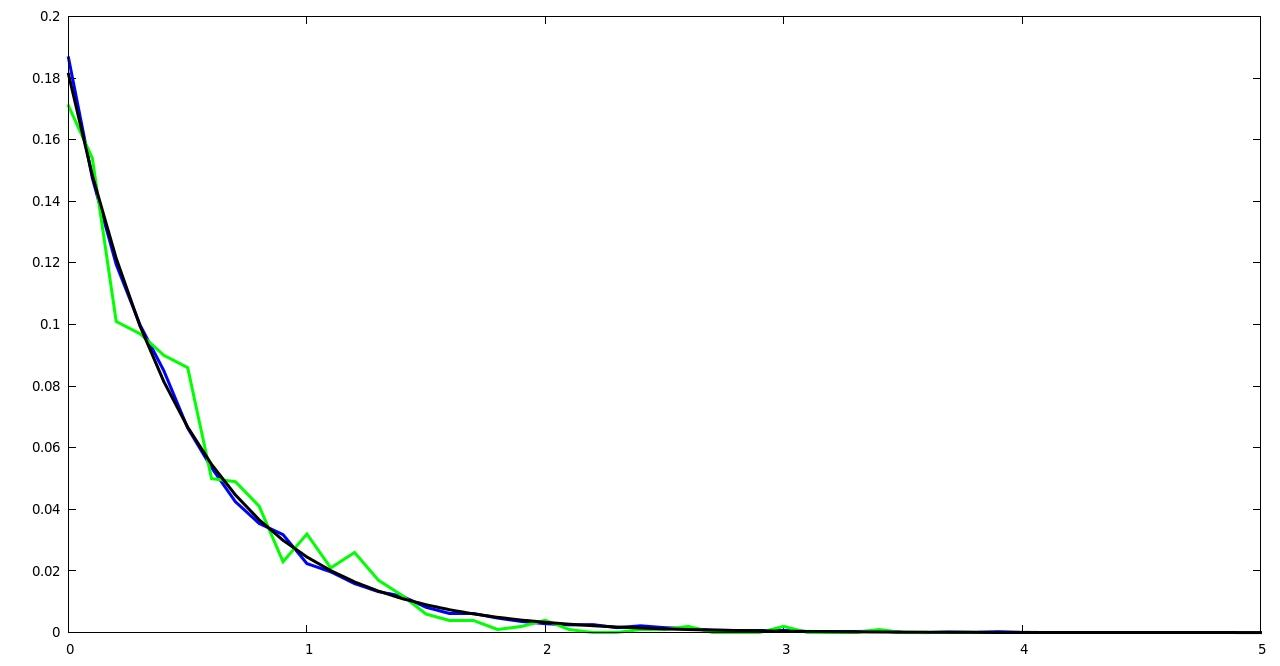
\includegraphics[width=\linewidth]{./img/Distribuicoes/expVarpt.jpg}
\caption{Variação no número de pontos da distribuição exponencial.}
\label{figExpPt}
\end{minipage} \hfill
\end{figure}


As curvas: vermelha e preta das figuras (\ref{figExpBar}) e (\ref{figExpPt}) representam variáveis aleatórias satisfazendo uma distribuição exponencial exata. Para plotar essas curvas foi utilizada a probabilidade da variável aleatória assumir um valor qualquer em um intervalo, tal probabilidade é dada pela frequência relativa:
\begin{equation}
f(X) = e^{-2x} - e^{-2(x+ 0.05)}.
\end{equation}

Após analisar a figura (\ref{figExpBar}), constatamos que a diminuição do número de barras faz a distribuição exponencial se deslocar em direção ao eixo X, já o aumento do número de barras  faz a curva se deslocar em direção contrária ao eixo X. Pode-se verificar essa asserção comparando as curvas: vermelha (ideal), verde (90 barras) e azul escuro (150 barras). 

Após análisar a figura (\ref{figExpPt}) observamos que a acurácia das curvas aumenta ou diminuí (em relação a curva preta) de acordo com o aumento ou redução do número de pontos utilizados para plotar as curvas. Para verificar esta asserção pode-se comparar as curvas: verde (1000pts), azul escuro (10000pts) e preto ($10^{8}pts$), observa-se que a curva azul (que possuí maior acurácia e número de pontos que a verde) possuí um comportamento mais próximo da curva rosa (ideal).

Codificamos em C  um algoritmo %(\ref{d_Gaussiana}) que gera uma variável aleatória que satisfaz uma Gaussiana normal de média 0 e variância 1 (N(0,1)) e  cuja FDP é:
\begin{equation}
FDP = \frac{1}{ \sigma  \sqrt{2 \pi } } e^{ \frac{-(x - \mu )^{2}}{{2 \sigma ^{2}}}}
\end{equation}
A variável aleatória satisfazendo uma distribuição Gaussiana com média 0 e variância 1, é de importância crucial para nosso trabalho. O movimento Browniano utiliza uma Gaussiana para gerar seus pontos e o algoritmo de Euler Maruyama utiliza o movimento Browniano para solucionar o termo estocástico da equação %(\ref{Cubo}).

\begin{figure}[!htb]
\centering
\begin{minipage}[b]{0.9\linewidth}
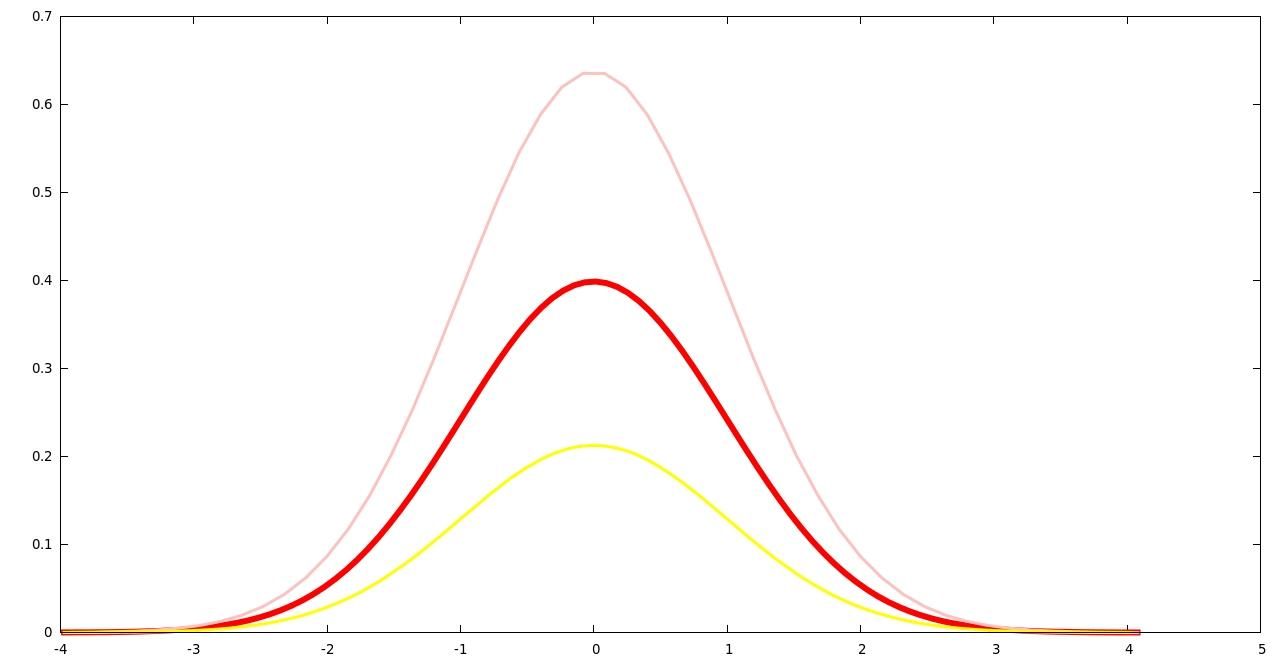
\includegraphics[width=\linewidth]{./img/Distribuicoes/GauVarBar.jpg}
\caption{Variação no número de barras da distribuição Gaussiana.}
\label{figGaussianaBar}
\end{minipage} \hfill
\end{figure}

\begin{figure}[!htb]
\centering
\begin{minipage}[b]{0.9\linewidth}
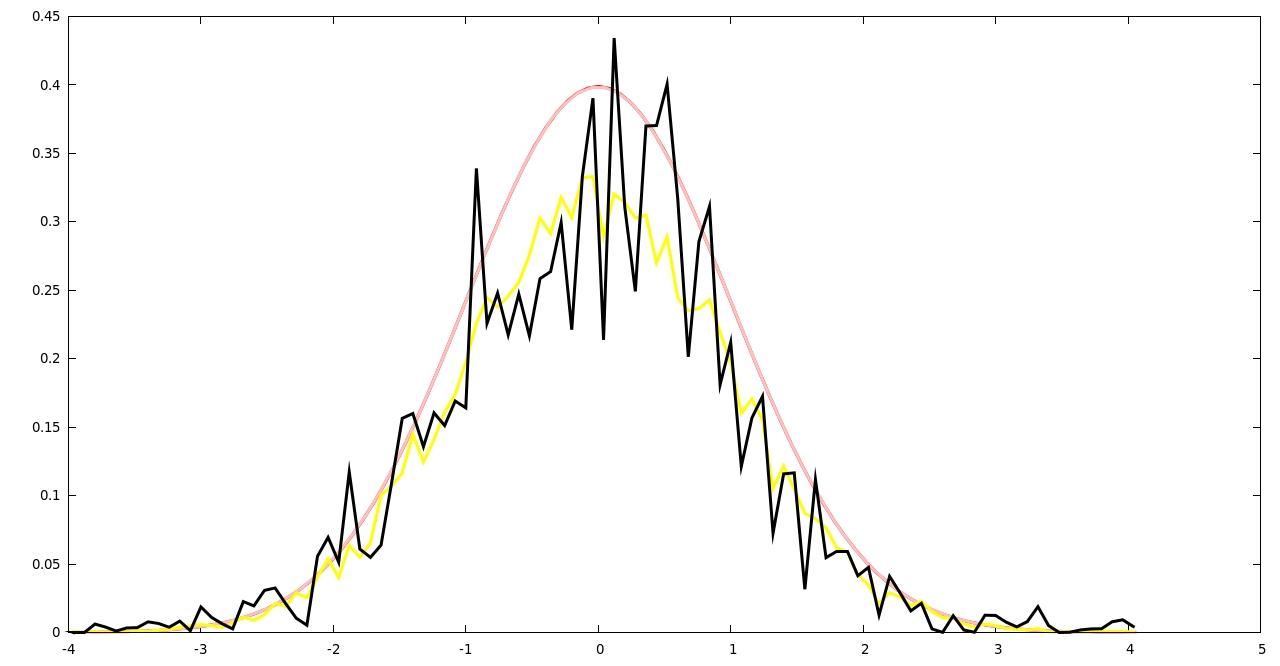
\includegraphics[width=\linewidth]{./img/Distribuicoes/GauVarPt.jpg}
\caption{Variação no número de pontos da distribuição Gaussiana.}
\label{figGaussianaPt}
\end{minipage} \hfill
\end{figure}

Obs.: As curvas vermelha e rosa das figuras (\ref{figGaussianaBar}) e (\ref{figGaussianaPt}) representam uma distribuição Gaussiana exata. Para plotar essas curvas foi utilizada a probabilidade da variável aleatória assumir um valor qualquer em um intervalo, tal probabilidade é dada pela frequência relativa da Gaussiana
\begin{eqnarray}
f(x) = \frac{1}{\sqrt{2 \pi}}exp(-\frac{x^{2}}{2})
\end{eqnarray}
Após analisar a figura (\ref{figGaussianaBar}) constatamos que a redução do número de barras faz a distribuição Gaussiana se deslocar em direção ao eixo X, um aumento do número de barras a desloca no sentido contrário ao eixo X. Essa constatação pode ser observada comparando as curvas vermelha (ideal), amarela (90 barras) e curva rosa (150 barras).
 
Atráves da figura (\ref{figGaussianaPt}) observamos que a acurácia das curvas aumenta ou diminuí (em relação a curva rosa) de acordo com o aumento ou redução do número de pontos utilizados para plotar as curvas. Para verificar esta asserção pode-se comparar as curvas: preta (1000pts), amarela (10000pts) e rosa ($10^{8}pts$), observa-se que a curva amarela (que possuí maior acurácia e número de pontos que a preta) possuí um comportamento mais próximo da curva rosa (ideal).	
\begin{figure}[!htb]
\centering
\begin{minipage}[b]{0.9\linewidth}
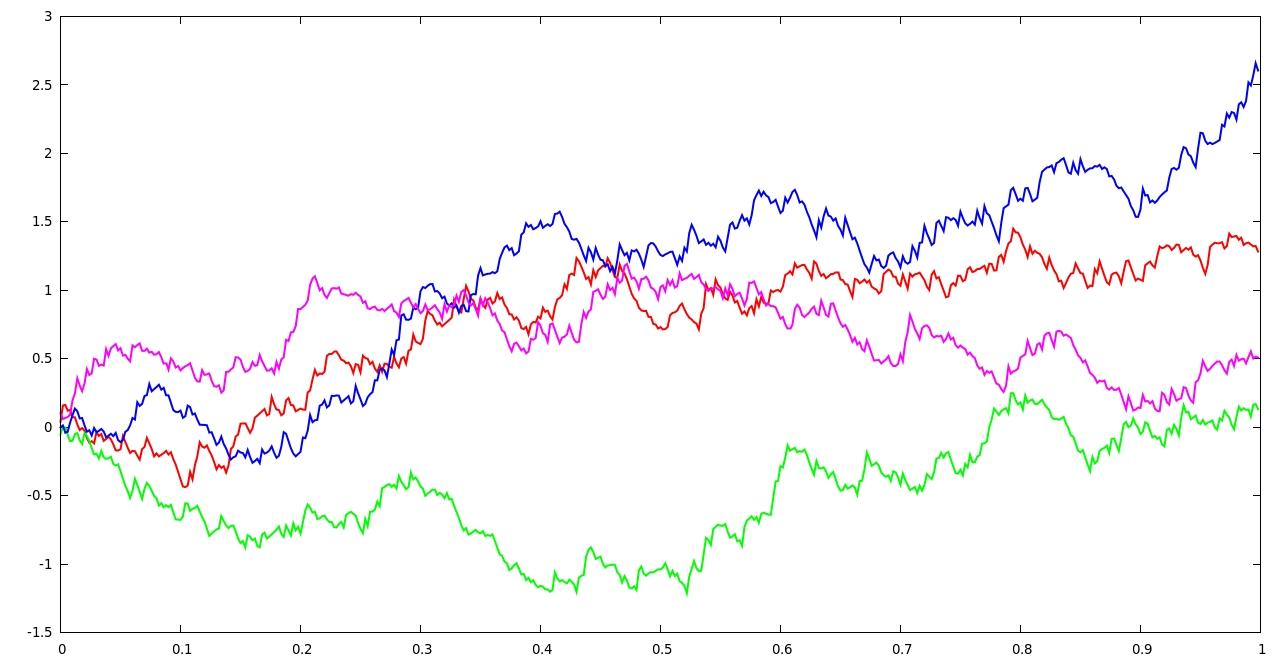
\includegraphics[width=\linewidth]{./img/Distribuicoes/Mb500pts.jpg}
\caption{Movimento Browniano com 500 pontos.}
\label{figMovBrown500}
\end{minipage} \hfill
\end{figure}

\begin{figure}[!htb]
\centering
\begin{minipage}[b]{0.9\linewidth}
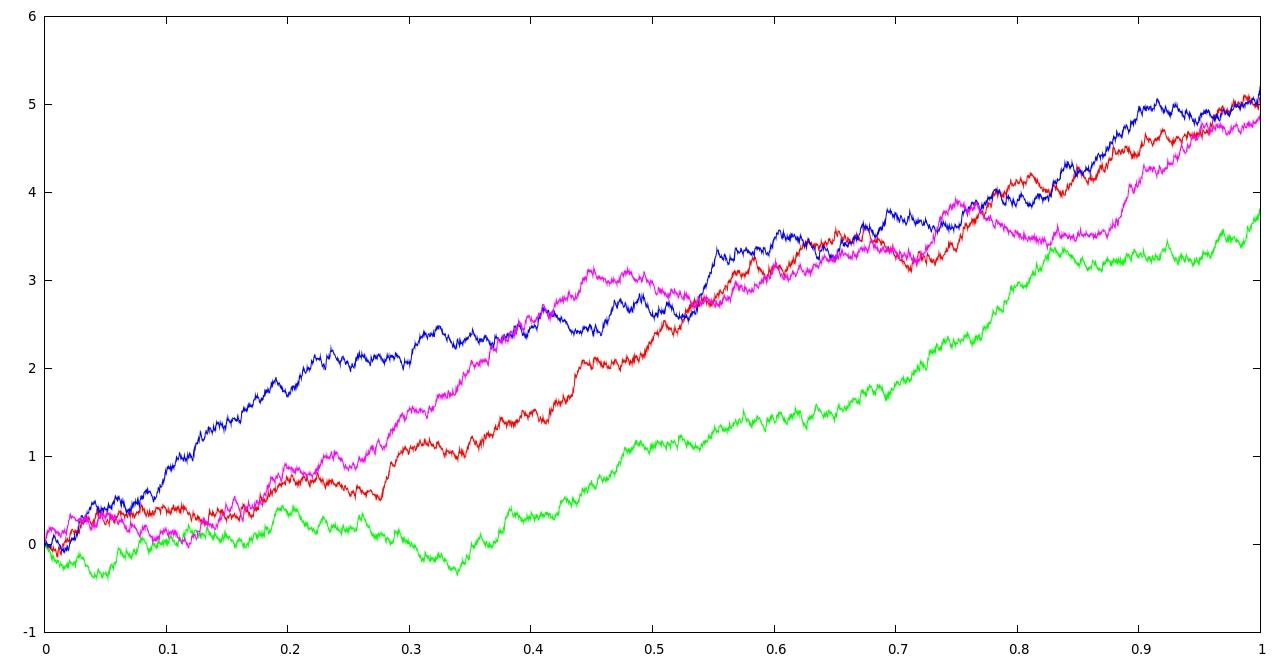
\includegraphics[width=\linewidth]{./img/Distribuicoes/MB5000ptos.jpg}
\caption{Movimento Browniano com 5000 pontos.}
\label{figMovBrown5000}
\end{minipage} \hfill
\end{figure}
Implementamos em C um algoritmo que gera o movimento Browniano %(\ref{movimentoBrownianoFONTE}) que utiliza uma variável aleatória Gaussiana de média 0 e variância 1 (N(0,1)). As figuras (\ref{figMovBrown500}) e (\ref{figMovBrown5000}) representam execuções do algoritmo que gera o movimento Browniano, as seguintes sementes aleatórias foram escolhidas: 34, 67, 157, 229. No caso da figura (\ref{figMovBrown500}), foram utilizados 500 pontos, a figura (\ref{figMovBrown5000}) utilizou 5000 pontos.